\section{Additional Results}
\label{appx:extra-results}

\subsection{Results with ``Oracle'' Retrieval}
\begin{table}
\centering
\begin{tabular}{lcc}
\toprule
\multirow{2}{*}{} & \multicolumn{2}{c}{``Oracle'' Retrieval} \\
\cmidrule(lr){2-3} 
Model & \% Resolved & \% Apply  \\
\midrule
Claude 2        & {\bf 4.80} & 62.82  \\
ChatGPT-3.5     & 0.52       & 21.80  \\
GPT-4$^*$       & 1.74       & 34.00  \\
SWE-Llama 7b    & 3.01       & 65.52  \\
SWE-Llama 13b   & 3.97       & {\bf 66.78}  \\
\bottomrule
\end{tabular}
\caption{
We compare models against each other using the oracle retrieval settings as described in Section~\ref{sec:experimental-setup}. The main results table, Table~\ref{table:main-results}, presents the results for the different models when using BM25 only. $^*$Due to budget constraints we evaluate GPT-4 on a $25$\% random subset of \benchmark{} in the ``Oracle" and BM25 27K retriever settings only.
}
\label{table:main-results-oracle}
\end{table}


% \begin{table}
% \centering
% \begin{tabular}{lcccc}
% \toprule
% \multirow{2}{*}{} & \multicolumn{2}{c}{BM25 Retrieval} & \multicolumn{2}{c}{``Oracle'' Retrieval} \\
% \cmidrule(lr){2-3} \cmidrule(lr){4-5} 
% Model & \% Resolved & \% Apply  & \% Resolved & \% Apply  \\
% \midrule
% Claude 2        & {\bf 1.96} & 43.07       & {\bf 4.80} & 62.82  \\
% ChatGPT-3.5     & 0.17       & 26.33       & 0.52       & 21.80  \\
% GPT-4$^*$       & 0.00       & 14.83       & 1.74       & 34.00  \\
% SWE-Llama 7b    & 0.70       & 51.74       & 3.01       & 65.52  \\
% SWE-Llama 13b   & 0.70       & {\bf 53.62} & 3.97       & {\bf 66.78}  \\
% \bottomrule
% \end{tabular}
% \caption{
% We compare models against each other using the BM25 and oracle retrieval settings as described in Section~\ref{sec:experimental-setup}. The main results table, Table~\ref{table:main-results}, presents the results for the different models when using BM25 only. $^*$Due to budget constraints we evaluate GPT-4 on a $25$\% random subset of \benchmark{} in the ``Oracle" and BM25 27K retriever settings only.
% }
% \label{table:main-results-oracle}
% \end{table}

Using the ``oracle'' retrieval method described in Section~\ref{sec:experimental-setup:input-formulation}, we show the general performance results in Table~\ref{table:main-results-oracle}. Naturally, providing only the files edited by the reference solution's pull request, model performance improves compared to the noisier BM25 retrieval setting.

\subsection{Evaluation Test Set}
\begin{table}[ht]
\begin{tabular}{lrrrrr}
    \toprule
    Repo & Claude 2 & ChatGPT-3.5 & GPT-4 & SWE-Llama $13$b & SWE-Llama $7$b \\
    \midrule
    astropy/astropy           & \num{3.23}  & \num{0.00} & \num{0.00} & \num{1.06 } & \num{3.16 } \\
    django/django             & \num{6.15}  & \num{1.32} & \num{2.50} & \num{5.19 } & \num{4.00 } \\
    matplotlib/matplotlib     & \num{3.05}  & \num{3.33} & \num{0.00} & \num{3.12 } & \num{1.11 } \\
    mwaskom/seaborn           & \num{0.00}  & \num{0.00} & \num{0.00} & \num{0.00 } & \num{0.00 } \\
    pallets/flask             & \num{0.00}  & \num{0.00} & \num{0.00} & \num{9.09 } & \num{0.00 } \\
    psf/requests              & \num{15.91} & \num{2.33} & \num{8.33} & \num{13.64} & \num{18.18} \\
    pydata/xarray             & \num{6.90}  & \num{0.00} & \num{0.00} & \num{5.81 } & \num{3.00 } \\
    pylint-dev/pylint         & \num{1.75}  & \num{0.00} & \num{0.00} & \num{1.75 } & \num{1.75 } \\
    pytest-dev/pytest         & \num{5.93}  & \num{0.00} & \num{0.00} & \num{5.04 } & \num{4.20 } \\
    scikit-learn/scikit-learn & \num{5.41}  & \num{0.00} & \num{0.00} & \num{3.12 } & \num{0.88 } \\
    sphinx-doc/sphinx         & \num{5.65}  & \num{1.83} & \num{0.00} & \num{2.25 } & \num{2.69 } \\
    sympy/sympy               & \num{1.94}  & \num{0.00} & \num{0.00} & \num{3.01 } & \num{1.59 } \\
    \bottomrule
\end{tabular}
\caption{\% Resolved for models per repository represented in \benchmark{}.}
\label{table:main-results-repo}
\end{table}
We include a repository-by-repository breakdown of model performance in Table~\ref{table:main-results-repo} that corresponds to Figure~\ref{fig:per-repo-oracle-fig} in the main paper. As discussed, in the main paper, performance differs heavily across repositories.

\subsection{GPT-4 Evaluation Subset Results}
In this section, we present the statistics shown in Table~\ref{table:main-results} for the $25$\% random subset that GPT-4 was tested in Table~\ref{table:main-results-20}.
As the selection of the subset is random, we find that the \% Resolved and \% Apply rates are consistent with the main results, and not significantly skewed towards being simpler or more difficult than the general evaluation set.

\definecolor{forestgreen}{RGB}{52,194,48}

\begin{table}[ht]
\centering
\begin{tabular}{lrrrr}
\toprule
\multirow{2}{*}{} & \multicolumn{2}{c}{BM25 Retrieval} & \multicolumn{2}{c}{``Oracle'' Retrieval} \\
\cmidrule(lr){2-3} \cmidrule(lr){4-5} 
Model & \% Resolved & \multicolumn{1}{c}{\% Apply} & \% Resolved & \% Apply  \\
\midrule
Claude 2       & 2.27 \textcolor{forestgreen}{$\uparrow 0.31$} & 45.72 \textcolor{forestgreen}{$\uparrow 2.65$} & 4.01 \textcolor{red}{$\downarrow 0.79$} & 62.65 \textcolor{red}{$\downarrow 0.17$} \\
ChatGPT-3.5    & 0.17 \textcolor{gray}{$- 0.00$} & 26.53 \textcolor{forestgreen}{$\uparrow 0.02$} & 0.70 \textcolor{forestgreen}{$\uparrow 0.18$} & 21.64 \textcolor{red}{$\downarrow 0.16$} \\
GPT-4          & 0.00 \textcolor{gray}{$- 0.00$} & 14.82 \textcolor{gray}{$- 0.00$} & 1.74 \textcolor{gray}{$- 0.00$} & 34.00 \textcolor{gray}{$- 0.00$} \\
SWE-Llama 7b   & 0.35 \textcolor{forestgreen}{$\uparrow 0.35$} & 49.04 \textcolor{red}{$\downarrow 2.70$} & 1.92 \textcolor{red}{$\downarrow 1.09$} & 63.70 \textcolor{red}{$\downarrow 1.82$} \\
SWE-Llama 13b  & 0.70 \textcolor{gray}{$- 0.00$} & 56.54 \textcolor{forestgreen}{$\uparrow 2.92$} & 4.54 \textcolor{forestgreen}{$\uparrow 0.57$} & 66.67 \textcolor{red}{$\downarrow 0.11$} \\

\bottomrule
\end{tabular}
\caption{
We compare models against each other using the BM25 and oracle retrieval settings as described in Section~\ref{sec:experimental-setup} on a $25$\% random subset (574 instances) of \benchmark{} in the ``oracle" and BM25 27K retriever settings only. This is the same subset that GPT-4 is evaluated on, as mentioned in Table~\ref{table:main-results}. The difference relative to percentages in Table~\ref{table:main-results} and Table~\ref{table:main-results-oracle} is included as a subscript.
}
\label{table:main-results-20}
\end{table}

% \textcolor{forestgreen}{$\uparrow 0.31$}
% \textcolor{red}{$\downarrow 2.46$}
% \textcolor{gray}{$- 0.00$}

\subsection{Extended Temporal Analysis}

In this section, we present an extended temporal analysis of task instances solved by year that follows the analysis shown in Table~\ref{table:temporal-results} of the evaluation section in the main paper.
In Table~\ref{appx:temporal-results-extended}, we present the \% Resolved statistic across models under the ``Oracle" retrieval setting for $6$ different temporal partitions that group tasks by the years in which the issues were created.
It is evident from the table that there is no consistent correlation between model performance and year, supporting our conclusion that despite having potentially seen older versions of code within its pre-training datasets, understanding and implementing in fixes in \benchmark{} is a difficult task that requires understanding and cannot be accomplished feasibly or consistently via memoization of observed data.

\begin{table}[ht]
\centering
\begin{tabular}{lcc|ccccc}
\toprule
    Year & Total & 25\% & Claude 2 & GPT-3.5 & GPT-4$^*$ & SWE-Llama 13b & SWE-Llama 7b \\
\midrule
    2023        & 244 & 61  & 4.51 & 1.56 & 0.00 & 4.07 & 3.50 \\
    2022        & 395 & 117 & 4.05 & 0.85 & 3.42 & 2.80 & 2.46 \\
    2021        & 383 & 102 & 4.18 & 0.00 & 2.94 & 4.45 & 2.56 \\
    2020        & 427 & 109 & 5.15 & 0.71 & 0.00 & 3.96 & 3.43 \\
    2019        & 437 & 112 & 5.72 & 1.49 & 1.79 & 4.55 & 2.21 \\
    2018        & 165 & 37  & 5.45 & 0.00 & 0.00 & 3.57 & 2.94 \\
    $<$ 2018 & 89  & 36  & 4.49 & 0.00 & 2.78 & 3.37 & 1.09 \\
\bottomrule
\end{tabular}
\caption{
We present an extended temporal analysis in this table, showing the \% resolved for task instances across models in the ``Oracle" retrieval setting, separated by different cutoff dates. The \textit{Year} column refers to the subset of tasks that were created during the specified calendar year. In the \textit{Total} column, we list the number of tasks that fall within the given year. The \textit{$25$\%} column is the same information for the subset that GPT-4 was evaluated on. The remaining model-specific columns contain the \% resolved metric.
}
\label{appx:temporal-results-extended}
\end{table}

\subsection{F2P, P2P Rate Analysis}

In the main paper results, we present the ``\% Resolved" statistic that indicates how many task instances were \textit{completely} solved by the different models.
In this section, we provide more fine-grained insight into the gap of task instances where 1. The model's patch generation was applied successfully and 2. The task instance was not resolved.
Assuming a patch is applied successfully, we define $6$ cases in Table~\ref{table:six-outcome-cases} that fully capture the distribution of all possible outcomes based on the pass/fail results of F2P and P2P tests.
In addition to the ``Resolved" outcome that has been established, we introduce five new terms.
The ``Breaking Resolved" outcome refers to when the desired behavior of the issue has been accomplished (all F2P tests pass), but not all prior behavior is maintained (not all P2P tests pass).
``Partially Resolved" refers to when prior behavior of a codebase was maintained (all P2P tests pass); however, the desired behavior is not fully accomplished (not all F2P tests pass).
The ``Work in Progress" case is when the desired behavior is not fully accomplished (not all F2P tests pass) and the prior behavior of the codebase is not maintained (not all P2P tests pass).
A ``No-Op" is when a code change does not have any effect on the original codebase; prior behavior is maintained (all P2P tests pass) but the issue remains completely unresolved ($0$ F2P tests pass).
Finally, if the issue is unresolved ($0$ F2P tests pass) and prior working behavior is reverted (some P2P tests fail), the codebase is left in a worse state, which we define to be a ``Regression".

\definecolor{green1}{RGB}{3,102,8}
\definecolor{green2}{RGB}{37,141,40}
\definecolor{green3}{RGB}{82,198,85}
\definecolor{green4}{RGB}{102,221,160}

\begin{table}[ht]
    \centering
    \begin{tabular}{l|ccc}
    \toprule
            & \multicolumn{3}{c}{\# F2P Tests Pass} \\
    \cmidrule(lr){2-4} 
    \# P2P Tests Pass & All               & Partial            & None \\
    \midrule
        All & \textcolor{green1}{Resolved} & \textcolor{green3}{Partially Resolved} & No-Op  \\
    Partial & \textcolor{green2}{Breaking Resolved} & \textcolor{green4}{Work in Progress} & \textcolor{red}{Regression} \\
       None & \textcolor{green2}{Breaking Resolved} & \textcolor{green4}{Work in Progress} & \textcolor{red}{Regression} \\
    \bottomrule
    \end{tabular}
    \caption{We present the 6 possible outcomes for a patch generation that is applied successfully and then executed. The outcomes are distinguished by the number of F2P and P2P tests that pass.}
    \label{table:six-outcome-cases}
\end{table}


In Table~\ref{table:six-outcome-stats}, we categorize patch generations that successfully applied according to these six cases.
We find that of non-``Resolved" issues, the majority of patch generations proposed by the model do not solve a single F2P test case from the corresponding task instance (``No-Op" and ``Regression").
Within the subset of these cases, the majority ($60\%$ to $70\%$) of cases are a No-Op, while the model breaks existing behavior for the remainder of these situations.

\begin{table}[ht]
    \centering
    \begin{tabular}{l|ccccc}
    \toprule
Model & Claude 2 & ChatGPT-3.5 & GPT-4$^*$ & SWE-Llama 7b & SWE-Llama 13b \\
    \midrule
Applied & 1078 & 284 & 76 & 1257 & 1196 \\
    \midrule
\textcolor{green1}{Resolved} & 110 & 12 & 10 & 69 & 91 \\
\textcolor{green2}{Breaking Resolved} & 26 & 2 & 3 & 17 & 10 \\
\textcolor{green3}{Partially Resolved} & 15 & 4 & 3 & 17 & 10 \\
\textcolor{green4}{Work in Progress} & 20 & 2 & 1 & 17 & 16 \\
No-Op & 471 & 174 & 30 & 716 & 672 \\
\textcolor{red}{Regression} & 436 & 90 & 29 & 421 & 397 \\
    \bottomrule
    \end{tabular}
    \caption{Categorization of model generations that applied successfully by the cases defined in Table~\ref{table:six-outcome-cases}. As mentioned, GPT-4 was evaluated on a $25$\% subset (574 instances) of \benchmark{}.}
    \label{table:six-outcome-stats}
\end{table}

Generally, the cases where model generations pass some, but not all tests (``Breaking Resolved", ``Partially Resolved", ``Work in Progress") cumulatively represent a smaller subset of problems relative to the other three categories.
From manual inspection of several of these cases, it is clear that the model demonstrates some understanding of the task requirements.
However, due to the baseline methods' limited view of the codebase that does not include information such as inter-file dependencies and functions' relationships, for many of these task instances often fail because a change that correctly resolves the immediate issue does not account for other modules that use and are affected by the changed entity.
We include several case studies that directly highlight these shortcomings in Section~\ref{appx:extra-results:quality-in-depth}
Overall, these results highlight not just the difficulty of \benchmark{}, but also point to the potential value of providing feedback via an execution environment that would allow models to run fixes against existing tests, then decide whether to continue editing or submit the patch for review.

\subsection{Patch Generation Extended Analysis}
In this section, we present a statistics to quantify various facets of patch generations following the metrics laid out in Table~\ref{table:quantitative-analysis-gens}.
In Table~\ref{table:quantitative-analysis-gens-all}, we recalculate these values for \textit{all} patch generations in the oracle retrieval setting for all models, regardless of whether or not the patch was applied successfully.
Across all metrics, we find that patch generations across models are much closer in size to the characteristics of average gold edits.
While some models still generate fewer lines relative to the corresponding Gold edit (e.g., Claude-2, ChatGPT-3.5, GPT-4), the SWE-Llama models edits are on average longer in most respects..
When considering both Table~\ref{table:quantitative-analysis-gens} and Table~\ref{table:quantitative-analysis-gens-all}, it becomes clear that models struggle with generating longer output sequences to be correctly formatted patches.
Further inspection of such occurrences, as shown in our case studies in Section~\ref{appx:extra-results:quality-in-depth}, indicate that hallucinations, abiding to existing code style/structure, and referencing long range dependencies correctly are common errors that surface more frequently in longer generations.

\begin{table}[ht]
\centering
\caption{
Average edits of model generated patches in the oracle retrieval setting across all patches (including unsuccessfully applied patches).
For the task instances specific to each model, we calculate the same statistics across the gold patches.
}
\begin{tabular}{lccccc}
\toprule
    Model & Total Lines & Added & Removed & Functions & Files \\ \cmidrule(lr){1-1} \cmidrule(lr){2-6}  
    Claude 2 & 27.2 & 6.6 & 3.3 & 1.2 & 1.1 \\
    \quad Gold & 61.6 & 17.8 & 8.6 & 2.6 & 1.4 \\
\midrule
    ChatGPT-3.5 & 42.0 & 6.1 & 3.9 & 1.7 & 1.0 \\
    \quad Gold & 44.5 & 12.7 & 5.5 & 2.1 & 1.2 \\
\midrule
    GPT-4 & 22.4 & 4.4 & 1.8 & 0.8 & 0.9 \\
    \quad Gold & 50.3 & 14.0 & 6.5 & 2.3 & 1.3 \\
\midrule
    SWE-Llama 13b & 68.9 & 9.5 & 4.3 & 2.5 & 1.6 \\
    \quad Gold & 61.5 & 17.8 & 8.6 & 2.6 & 1.4 \\
\midrule
    SWE-Llama 7b & 78.9 & 10.1 & 7.6 & 2.5 & 1.5 \\
    \quad Gold & 65.1 & 18.8 & 9.0 & 2.7 & 1.5 \\
\bottomrule
\end{tabular}
\label{table:quantitative-analysis-gens-all}
\end{table}

\subsection{Software Engineering Metrics}
We perform preliminary evaluations that explore using \textit{software engineering} metrics to evaluate the efficiency and complexity of large code blocks integrated within a complex codebase.
Unlike semantic similarity scoring functions for evaluating fluency and surface form likeness that are popular with traditional NLP benchmarks and have been adopted for code generation, metrics such as Cyclomatic complexity~\cite{mccabe1976complexity} and Halstead complexity measures~\cite{Halstead1977ElementsOS} are founded upon logical abstractions (e.g., Abstract Syntax Trees) and software principles to quantify the complexity, efficiency, and readability of code as a scalar value.
The patch generations and \benchmark{} evaluation logs are rich sources of information that software engineering metrics and static analyzers can readily be applied to.
Unlike small, code contest benchmarks where the insights of software engineering metrics are not meaningful due to the minuscule scope of the target functionality, \benchmark{}'s task is complex enough that practitioners can use these tools to gain well-structured, rigorous, and wide-ranging feedback signals on the complexity of a patch generation's change and its effect on the rest of the codebase.

\begin{table}[t]
\centering
\small
\begin{tabular}{p{0.9\linewidth}}
    \toprule
    \textbf{Problem Statement}: Misleading exception with invalid protocol in proxy variable. When the value of \texttt{https\_proxy} or \texttt{HTTPS\_PROXY} variable(s) accidentally miss one '/' in the protocol, a traceback is thrown to the user which doesn't pin point that the issue is with the proxy configuration... \\
    \bottomrule
    \vspace{1em}
\end{tabular}
\begin{minipage}{.44\linewidth}
    \begin{minipage}{\textwidth}
        \centering
        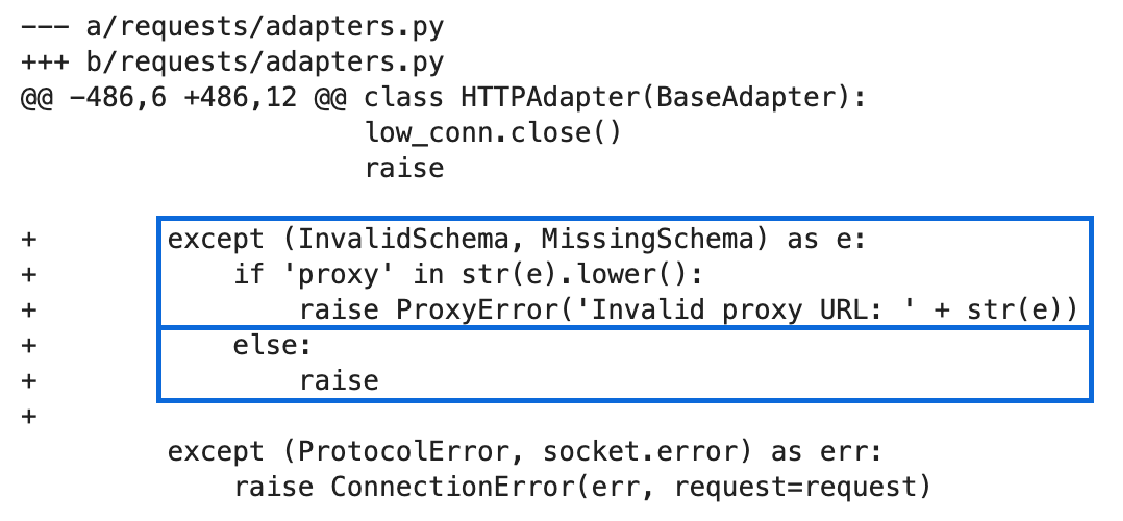
\includegraphics[width=\textwidth]{figures/assets/swe-metrics-pred.pdf}
    \end{minipage}
\end{minipage}
\hfill
\begin{minipage}{.55\linewidth}
    \begin{minipage}{\textwidth}
        \centering
        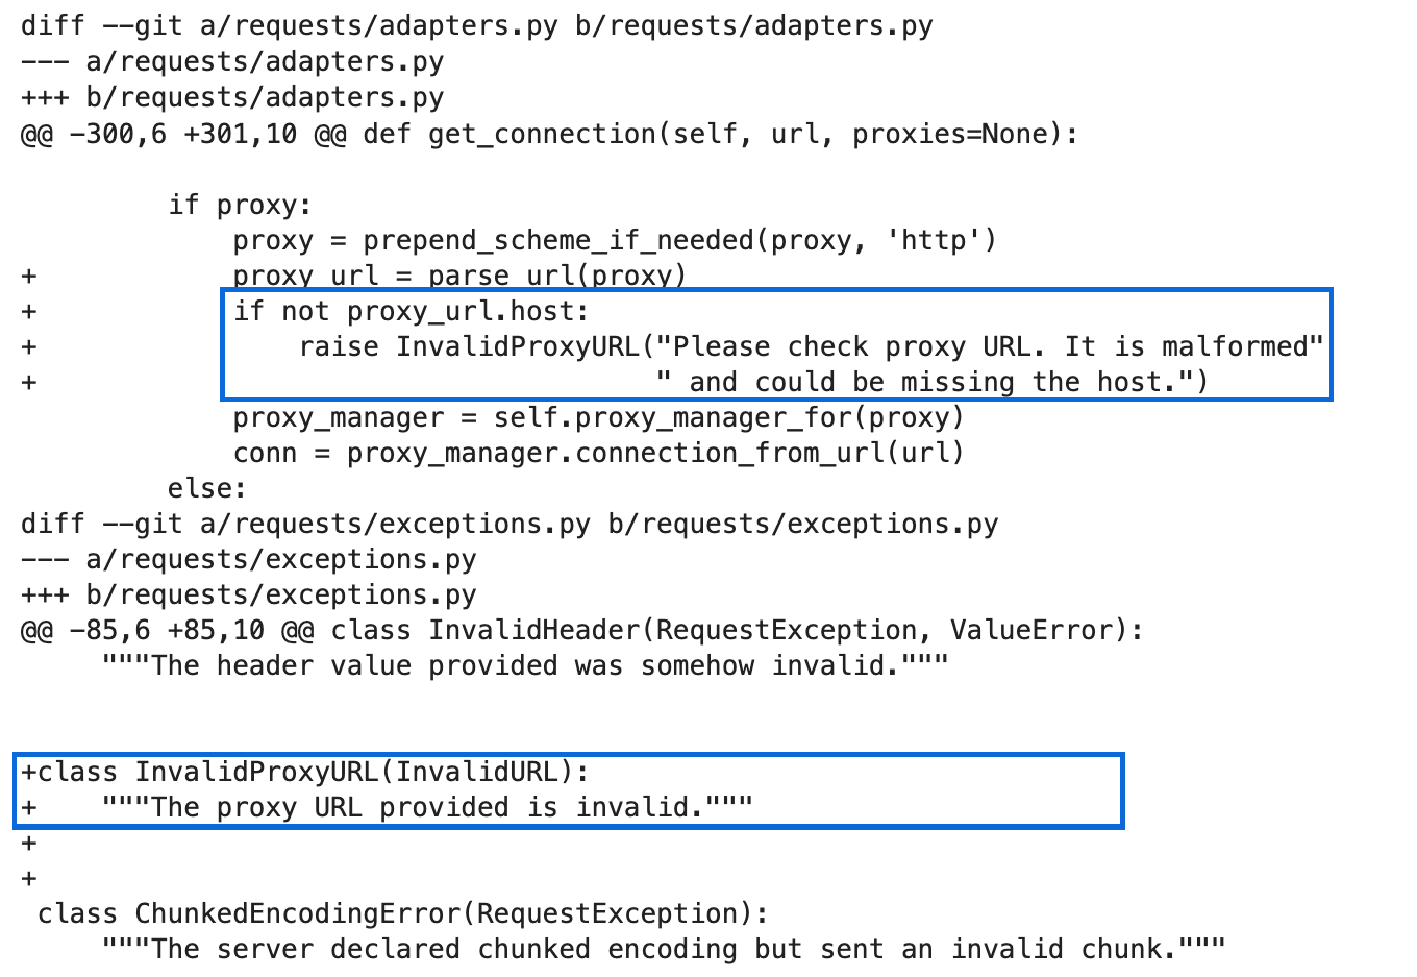
\includegraphics[width=\textwidth]{figures/assets/swe-metrics-gold.pdf}
    \end{minipage}
\end{minipage}
\captionof{figure}{Comparison of the Claude 2 prediction (left) and reference solution (right) patches for \benchmark{} task instance \texttt{psf\_\_requests-4356}. While the code generated by the patch is fewer lines of code and solves the problem correctly, the prediction patch introduces greater Cyclomatic complexity (\texttt{requests.adapters.py/HTTPAdapter}: 3 $\rightarrow$ 5) compared to the gold solution (\texttt{requests/adapters.py:get\_connection}: 2 $\rightarrow$ 3, \texttt{requests/exceptions.py:InvalidHeader}: 0 $\rightarrow$ 1). Changes that introduce new execution paths are boxed in blue. Parts of the gold patch have been truncated for appearance.}
\label{fig:swe-metrics-comparison}
\end{table}


We include our exploratory work here that demonstrates how software engineering metrics can reliably capture characteristics of code quality, and how comparing these statistics across two patches can provide automatic observations about model capabilities.
We use the Radon package\footnote{Radon \href{https://radon.readthedocs.io/en/latest/}{Documentation}, open-source \href{https://github.com/rubik/radon}{codebase}}, a library for computing different software engineering metrics directly from source code.

We look specifically at successfully applied Claude 2 patch predictions in the ``Oracle" retrieval setting for the \texttt{psf/requests} repository, which several models perform best at as reflected in Figure~\ref{fig:per-repo-oracle-fig}.
Per prediction, we apply the patch to the codebase, then calculate the Cyclomatic complexity and Halstead complexity scores for the modified functions.
Cyclomatic complexity quantifies the control flow of a function, counting the number of independent execution paths through the source code~\citep{mccabe1976complexity}.
A higher Cyclomatic complexity score suggests a more complex function that has higher likelihood of defects and usually suggests difficult maintainability.
Halstead complexity counts the number of operators and operands in a program~\citep{Halstead1977ElementsOS}.
Per prediction, we also perform the same set of steps for the corresponding gold patch.

We find that software engineering metrics provides automatic qualitative insights into model performance.
Consider the following simple case study in Figure~\ref{fig:swe-metrics-comparison}.
While the model patch prediction (left) is fewer lines ($6$ instead of $11$) and modifies fewer files ($1$ instead of $2$) compared to the gold reference solution (right), the model's edit places a conditional within a relatively complex and widely used \texttt{HTTPAdapter} class.
This introduces two new potential execution outcomes, raising the Cyclomatic complexity of \texttt{HTTPAdapter} from $3$ to $5$.
In contrast, while longer, the reference solution imports intra-module dependencies, modifies a logically simpler function in \texttt{get\_connection}, and defines a new error type \texttt{InvalidProxyURL} to capture the novel bug described by the issue.
